\chapter{Original methodology for the (computer aided) forensic audit}
\komentar{Jsem si vedoma, ze jsem clovek, ktery to nikdy nedelal (= omezena znalost).
Toto je jak to chapu. Toto neni jak by to nekdo mel delat. Toto je seriozni pokus popsat proces forenzniho auditu.
PROCESNI DIAGRAMY!!!

vystupem = okomentovany obrazek, ktery dava hlavu a patu

s Use case diagrammem pak kontaktovat praxi

}


We are aware to have only limited knowledge of forensic audit and no practical experience. This chapter should not be considered as a manual explaining how forensic audit should be done.  However, this is rather a serious attempt to describe the process of forensic audit.


\section{The phase of preparation of the forensic-audit process}
Before the process of forensic audit starts there is a block of organizational or administrative affairs that needs to be \anglictina{done}. It all starts in a institution where there is a suspicion of an act that is not following required rules. The institution might be of various kinds. A example can be an international corporation suspecting one of local branches from a money leakage. \komentar{dalsi priklady?}

The rules might be either internal regulation or corporate policies or even given by law. Basically any kind of misbehavior can be investigated by forensic audit. Given the background of the case the ordering party might also be of multiple kinds and from various branches of economy. They usually suspect possible internal or external risks that can be represented by fraudsters or people committing some other type of crime.  Generally the ordering party is the head of a given company. Some specific cases are: CEO of certain company, new holder of an existing company, authorized representative of a supervisory board etc.. However forensic audit can be also assigned by a court or the police. 

After the decision to perform forensic audit the ordering party contacts the audit company and they negotiate with a business representative about the sphere of the contract, price and deadlines. If there is no agreement it is probable that the ordering party contacts another audit company. If both parties agree the contract is made and the case is accepted. 

In the audit company there is a team of specialists established according to the character of the case. It is important to be aware of conflict of interest in this phase. Members of the team must not be related in any way to the original case. Members of the team can be forensic auditors, data analytics, specialists in any particular field (biometry, data recovery, criminology, law, etc.), consultants and assistants. 

When the team of auditors is established the next thing is creating a document for record of the investigation. It also serves as a documentation. This is the end of all the administration needed to be done before the actual forensic audit. 

\section{Accumulation of data}
In the beginning of the investigation the team needs to gain an insight into the background situation of the case. They can learn it from materials they have been provided by the client. An appropriate strategy for investigation is created. It means, that all the relevant methods are taken account of and the best are chosen. 

In all the cases it is important to secure all the documents, data repositories and all other possible sources of (digital) evidence. Any unauthorized person must not have a chance to manipulate with any possible evidence. For this reason backups of all the digital information are made. According to a FBI statistics the average investigated case size is approximately 500 GB. \komentar{citace (ariu- paper, zdroj 13)} In fact there are usually two copies of the data. The first is utterly for backup and the second can be used for work and analysis of the data. 






\colorbox{green}{\komentar{ timhle diagramem bude problem, budu ho muset prinutit aby se rozdelil na vic stran}}

\begin{figure}[h]
	\begin{center} 
	%\missingfigure{Velky obrazek vsech zainteresovanych stran - f.auditor, datovy analytik pro FA, zakaznik (zadavatel, materska spolecnost)}
	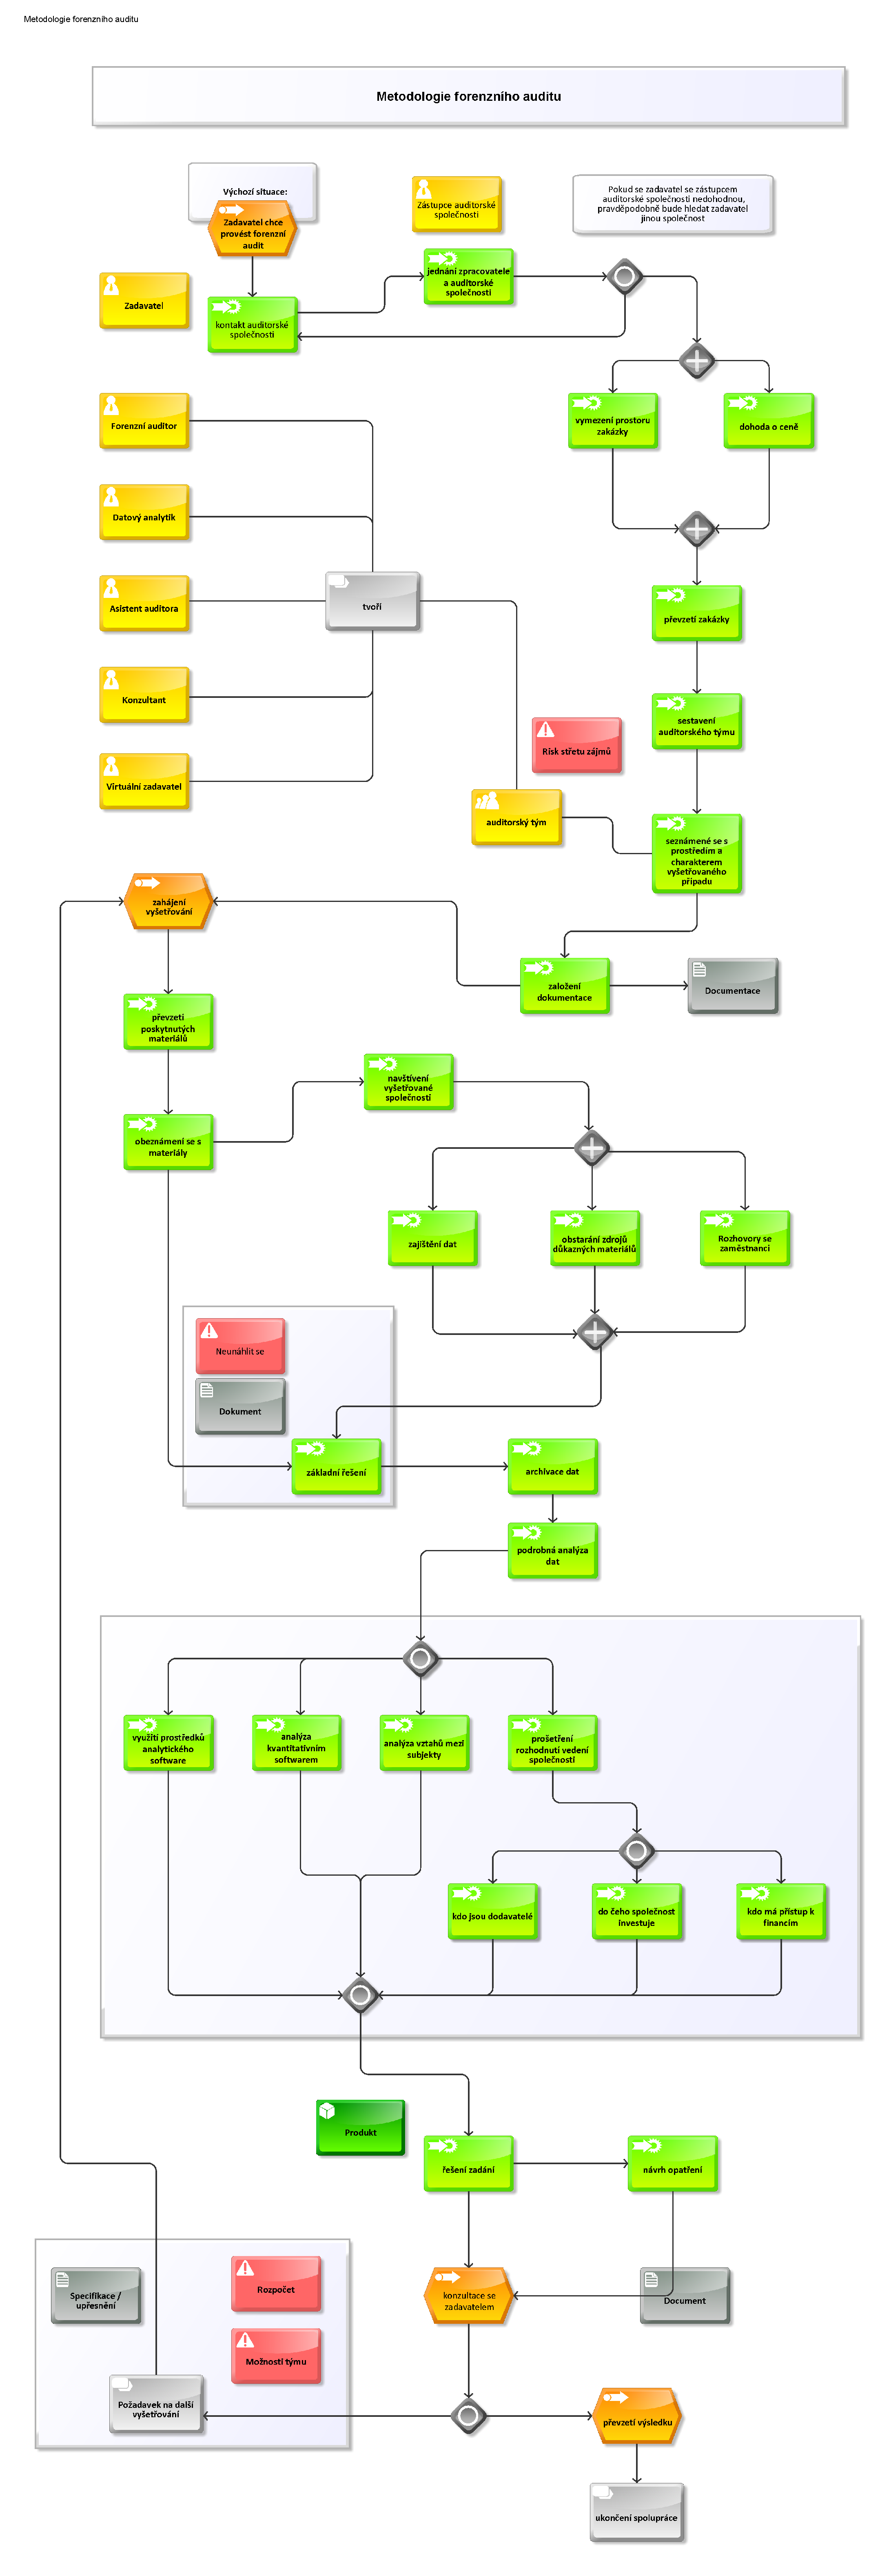
\includegraphics[width=1.0\textwidth]{img/metodika/Metodologie_forenzniho_auditu.pdf}
	\end{center}
	\caption{\komentar{Metodika v ARISu}}
\end{figure}

